\begin{frame}{$d(K^-, n \pi^+ \pi^-)"X"$ tail study by $\Sigma_{forwrad} \& K^0$ prod. }
  \centering
  CDSでの散乱が広いテールの成分を作る\\
  牛若での散乱は高い位置に分布する\\
  
  \tminipageThree{
    \begin{figure}
      \scriptsize
      $K^- d\rightarrow "n_{spec}" K^0 n$
      \includegraphics[width=4cm]{../pic/sim/KNpipi_MM_n_scat_K0.eps}
      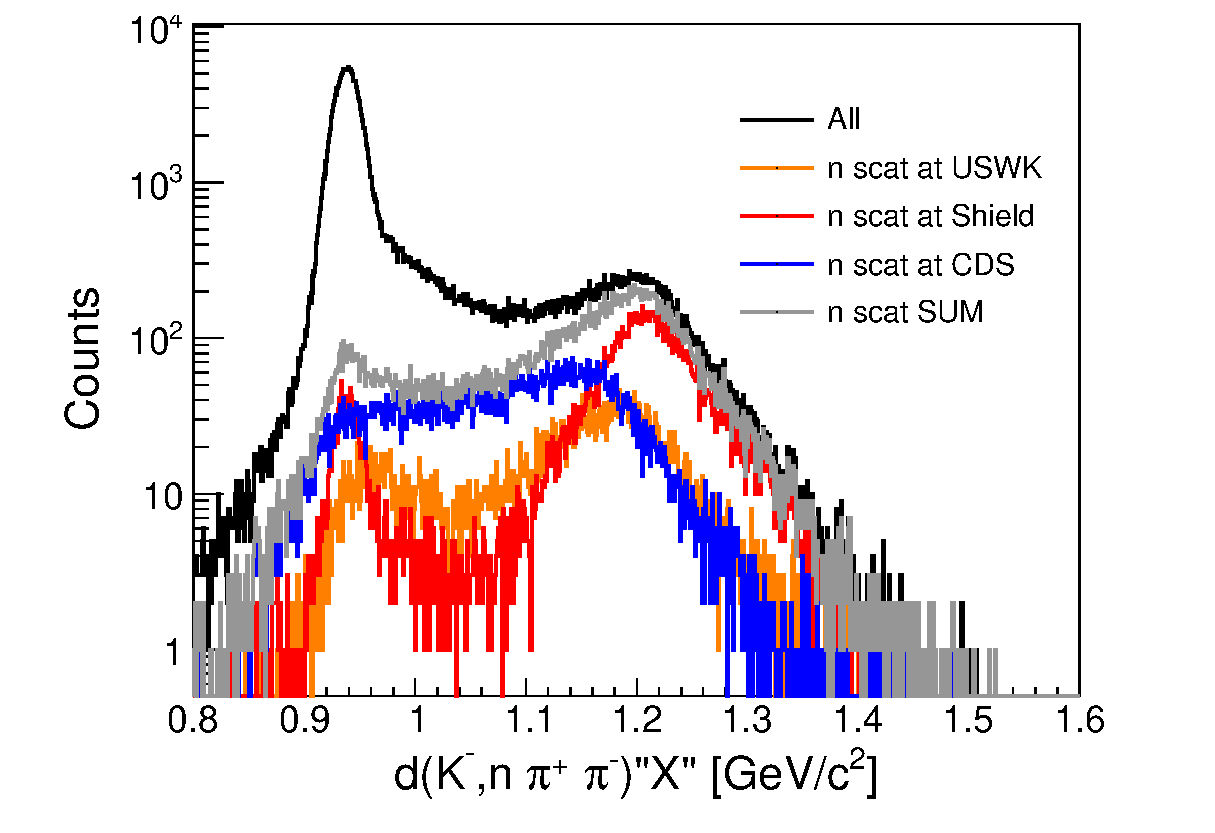
\includegraphics[width=4cm]{../pic/sim/KNpipi_MM_n_scat_K0_logy.eps}
    \end{figure}
  }{
    \begin{figure}
      \scriptsize
      $K^- d\rightarrow \pi^+ \Sigma^- n_{forward}$
      \includegraphics[width=4cm]{../pic/sim/KNpipi_MM_n_scat_pipSm.eps}
      \includegraphics[width=4cm]{../pic/sim/KNpipi_MM_n_scat_pipSm_logy.eps}
    \end{figure}
  }{
    \begin{figure}
      \scriptsize
      $K^- d\rightarrow "n_{spec}" \pi^- \Sigma^+_{forward}$
      \includegraphics[width=4cm]{../pic/sim/KNpipi_MM_n_scat_pimSp.eps}
      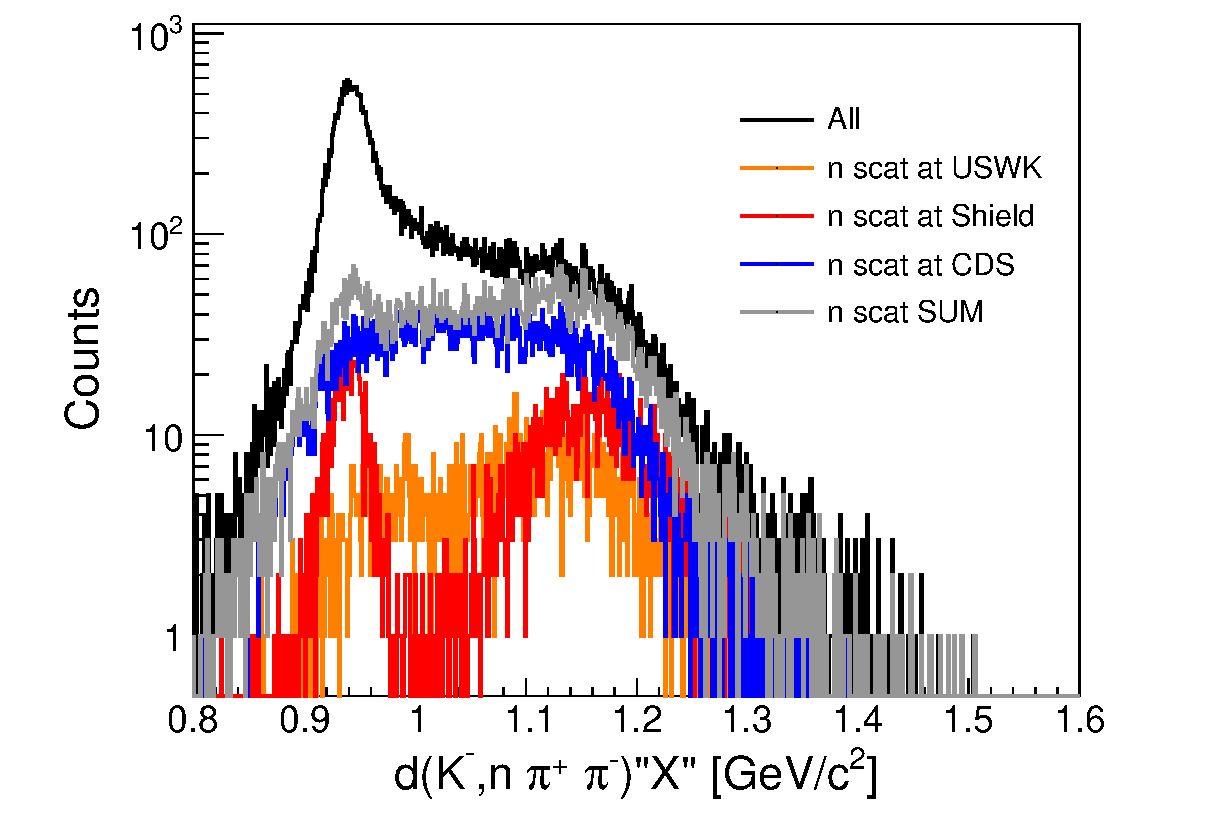
\includegraphics[width=4cm]{../pic/sim/KNpipi_MM_n_scat_pimSp_logy.eps}
    \end{figure}    
  }
\end{frame}
